\documentclass{standalone}

\usepackage{amsmath}
\usepackage{tikz}
\usepackage{mathdots}
\usepackage{yhmath}
\usepackage{cancel}
\usepackage{color}
\usepackage{siunitx}
\usepackage{array}
\usepackage{multirow}
\usepackage{amssymb}
\usepackage{gensymb}
\usepackage{tabularx}
\usepackage{booktabs}
\usetikzlibrary{fadings}
\usetikzlibrary{patterns}
\usetikzlibrary{shadows.blur}
\usetikzlibrary{shapes}

\begin{document}

\tikzset{every picture/.style={line width=0.75pt}} %set default line width to 0.75pt        

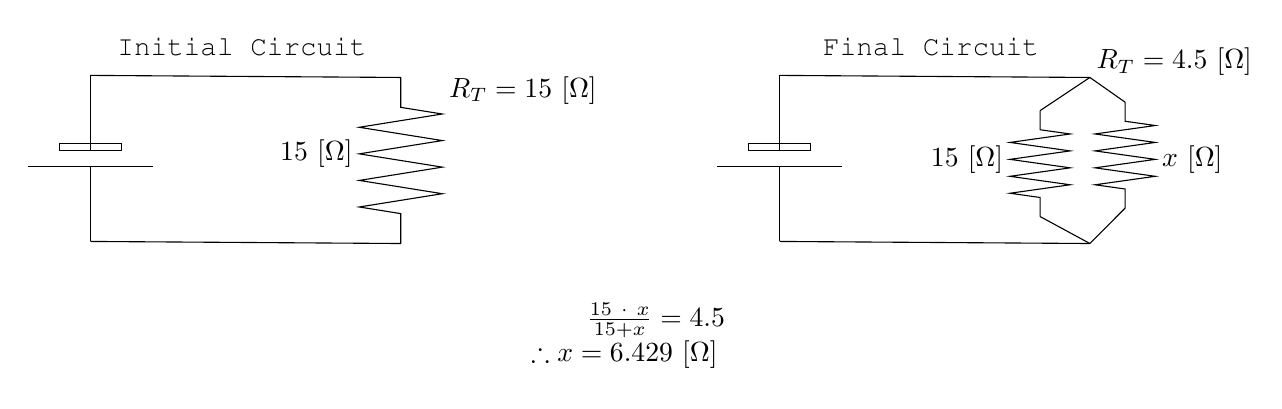
\begin{tikzpicture}[x=0.75pt,y=0.75pt,yscale=-1,xscale=1]
%uncomment if require: \path (0,300); %set diagram left start at 0, and has height of 300

%Shape: Resistor [id:dp06538230023270464] 
\draw   (183.5,130) -- (183.5,144.4) -- (203.5,147.6) -- (163.5,154) -- (203.5,160.4) -- (163.5,166.8) -- (203.5,173.2) -- (163.5,179.6) -- (203.5,186) -- (163.5,192.4) -- (183.5,195.6) -- (183.5,210) ;
%Shape: Battery [id:dp424752245476688] 
\draw   (34,129) -- (34,165) (64,173) -- (4,173) (34,173) -- (34,209) (49,161.8) -- (49,165) -- (19,165) -- (19,161.8) -- (49,161.8) -- cycle ;
%Straight Lines [id:da8724969604842278] 
\draw    (34,129) -- (183.5,130) ;
%Straight Lines [id:da6098746761706486] 
\draw    (34,209) -- (183.5,210) ;

%Shape: Resistor [id:dp3461605413423553] 
\draw   (491.5,146) -- (491.5,155.18) -- (506,157.22) -- (477,161.3) -- (506,165.38) -- (477,169.46) -- (506,173.54) -- (477,177.62) -- (506,181.7) -- (477,185.78) -- (491.5,187.82) -- (491.5,197) ;
%Shape: Battery [id:dp9842410846556896] 
\draw   (366,129) -- (366,165) (396,173) -- (336,173) (366,173) -- (366,209) (381,161.8) -- (381,165) -- (351,165) -- (351,161.8) -- (381,161.8) -- cycle ;
%Straight Lines [id:da5276602494962671] 
\draw    (366,129) -- (515.5,130) ;
%Straight Lines [id:da18191368096351368] 
\draw    (366,209) -- (515.5,210) ;
%Straight Lines [id:da6636941916823806] 
\draw    (515.5,130) -- (491.5,146) ;
%Straight Lines [id:da9312038302789695] 
\draw    (515.5,210) -- (491.5,197) ;
%Straight Lines [id:da6771483869404411] 
\draw    (532.5,141.92) -- (515.5,130) ;
%Straight Lines [id:da1563736652068749] 
\draw    (515.5,210) -- (532.5,192.92) ;
%Shape: Resistor [id:dp35484716983932996] 
\draw   (532.5,141.92) -- (532.5,151.1) -- (547,153.14) -- (518,157.22) -- (547,161.3) -- (518,165.38) -- (547,169.46) -- (518,173.54) -- (547,177.62) -- (518,181.7) -- (532.5,183.74) -- (532.5,192.92) ;


% Text Node
\draw (107,115) node   [align=left] {{\fontfamily{pcr}\selectfont Initial Circuit}};
% Text Node
\draw (161.5,166.8) node [anchor=east] [inner sep=0.75pt]    {$15\ [ \si{\ohm}]$};
% Text Node
\draw (205.5,144.2) node [anchor=south west] [inner sep=0.75pt]    {$R_{T} =15\ [ \si{\ohm}]$};
% Text Node
\draw (517.5,114.62) node [anchor=north west][inner sep=0.75pt]    {$R_{T} =4.5\ [ \si{\ohm}]$};
% Text Node
\draw (475,169.46) node [anchor=east] [inner sep=0.75pt]    {$15\ [ \si{\ohm}]$};
% Text Node
\draw (439,115) node   [align=left] {{\fontfamily{pcr}\selectfont Final Circuit}};
% Text Node
\draw (549,169.46) node [anchor=west] [inner sep=0.75pt]    {$x\ [ \si{\ohm}]$};
% Text Node
\draw (293,255) node    {$ \begin{array}{l}
\ \ \ \ \ \ \frac{15\ \cdotp \ x}{15+x} =4.5\\
\therefore x=6.429\ [ \si{\ohm}]
\end{array}$};

\end{tikzpicture}

\end{document}
